\chapter{Summary and Outlook}
\label{chap:outlook}

\section{Summary}
We have reported the newest dielectron measurements in U + U collisions at $\sqrt{s_{NN}}$ = 193 GeV by the STAR experiment at RHIC. The measured dielectron invariant mass spectrum within STAR acceptance ($p_{T}^{e}>0.2$ GeV/$c$, $|\eta^{e}|<$ 1, and $|y_{ee}|<$ 1) in minimum-bias collisions shows an enhancement with respect to hadronic cocktail simulation in the mass region 0.3-0.76 GeV/$c^{2}$ ($\rho$-like). The enhancement factor, integrated over the $\rho$-like mass region and the full $p_{T}$ acceptance, is 2.1 $\pm$ 0.1(stat.) $\pm$ 0.2(sys.) $\pm$ 0.3(cocktail). Meanwhile, systematic measurements are performed in differential $p_{T}$ bins and centrality bins. The enhancements in LMR are consistently observed and the enhancement factor has a mild $p_{T}$ and centrality dependence. An effective many-body model calculation (Rapp $et\,al.$) including a broadened $\rho$ spectral function and QGP thermal radiation is employed to compare with our measurements, which can reasonably describe these low-mass enhancements. The integrated excess yields in the $\rho$-like mass region increase faster than $N_{part}$ scaling as a function of centrality, indicating that the dielectron yields in the $\rho$-like region are sensitive to the QCD medium dynamics. Furthermore, the dielectron excess invariant mass spectra, with STAR acceptance corrected for, are reported for the first time in U + U collisions at $\sqrt{s_{NN}}$ = 193 GeV. The charged particle density normalized integral yields (in 0.4 $<M_{ee}<$ 0.75 GeV/$c^{2}$) of the most central U + U collisions at $\sqrt{s_{NN}}$ = 193 GeV are higher than those in peripheral or lower-energy collisions, which indicates that the hot and dense medium created in central U + U collisions at $\sqrt{s_{NN}}$ = 193 GeV has a longer lifetime.

We also report the dielectron mass spectra within STAR acceptance at very low $p_{T}$ ($p_{T}$ < 0.15 GeV/$c$) in U + U collisions at $\sqrt{s_{NN}}$ = 193 GeV. The dielectron yields show a significant enhancement with respect to hadronic cocktail for the entire mass region in the most peripheral (60-80\%) collisions. The enhancement factors are 16.4 $\pm$ 1.1(stat.) $\pm$ 2.6(sys.) $\pm$ 4.2(cocktail) and 20.4 $\pm$ 4.2(stat.) $\pm$ 3.0(sys.) $\pm$ 3.2(cocktail) in 0.4 $<M_{ee}<$ 0.76 GeV/$c^{2}$ and 2.8 $<M_{ee}<$ 3.2 GeV/$c^{2}$, respectively. Moreover, the $p_{T}$ spectra within STAR acceptance for three selected pair invariant mass regions (0.4 $<M_{ee}<$ 0.76 GeV/$c^{2}$, 1.2 $<M_{ee}<$ 2.67 GeV/$c^{2}$, and 2.8 $<M_{ee}<$ 3.2 GeV/$c^{2}$) are reported. The $p_{T}$ spectra have a fairly sharp transition around 0.1 GeV/$c$ in all the three mass regions in the most peripheral U + U collisions. These observed excess may be from the photoproduction in the peripheral collisions, which will provide insight into the dynamics of nuclear interactions and may become a novel probe of the QGP.

This thesis also presents the R\&D work on two different gaseous detectors: mini-drift THGEM and MRPC. Trough the cosmic ray test, the THGEM exhibits excellent performance. The detection efficiency of the THGEM chamber is greater than 94$\%$ and the 1-D spatial resolution is $\sim$220 $\mu$m. Furthermore, the THGEM chamber shows excellent track reconstruction capability and good uniformity and stability, which are essential to the TRD design. Three MRPC prototypes with different readout modes (single-end and double-end readout modes) show remarkable performance in the beam test. The efficiencies of all three MRPC modules are higher than 98\%. The time resolution of single-end readout MRPC is 47 ps but has incident position dependence. The time resolution of double-end readout MRPC is 40 ps and the double-end readout MRPC is insensitive to the position of incidence. The double-end readout MRPC is finally decided to be used for the Beijing Spectrometer eTOF upgrade according to this beam test. In November 2015, the MRPC-based eTOF system was fully installed in Beijing Spectrometer. The time resolution of the MRPC-based eTOF system obtained from the collision data is $\sim$60 ps, which is much better than the design specification (80 ps).

\section{Outlook}
A major goal of heavy-ion collisions is to determine the QCD phase diagram which is a unique and fundamental feature of Quantum Chromodynamics (QCD). The most experimentally accessible way to characterize the QCD phase diagram is in the plane of temperature ($T$) and the baryon chemical potential ($\mu_{B}$). In order to study experimentally the QCD structure as a function of $T$ and $\mu_{B}$, the first RHIC Beam Energy Scan (BES \uppercase\expandafter{\romannumeral1})~\cite{BESI} was carried out in which data were acquired from Au + Au collisions at energies of 62.4, 39, 27, 19.6, 14.5, 11.5 and 7.7 GeV in years 2010, 2011 and 2014. The results from BES \uppercase\expandafter{\romannumeral1} of searching for the critical point and first-order phase boundary have narrowed the region of interest to collision energies below $\sqrt{s_{NN}}$ = 20 GeV. The BES \uppercase\expandafter{\romannumeral1} data also enabled other new and systematic measurements, such as the dielectron mass spectrum in the LMR, which is considered to be a link to chiral symmetry restoration. However, the strength of the conclusions is limited by statistical and systematic uncertainties in the measurements of BES \uppercase\expandafter{\romannumeral1} program. BES \uppercase\expandafter{\romannumeral2} has been proposed based on the results from BES \uppercase\expandafter{\romannumeral1}, aiming for collecting high-statistics data at the lower-energy end of the BES \uppercase\expandafter{\romannumeral1} range ($\sqrt{s_{NN}}$ < 20 GeV) with the electron cooling~\cite{ecooling} upgrade to the collider. The electron cooling upgrade to the collider will increase the luminosity for future low energy runs by a factor of four to fifteen. Meanwhile, two sub-systems (inner Time Projection Chamber and end-cap Time of Flight) of STAR will be upgraded, which will significantly improve the quality of the measurements. BES \uppercase\expandafter{\romannumeral2} is scheduled to run in years 2019 and 2020~\cite{BESII}, and focuses on the low collision energies which cover the range from 7.7 to 19.6 GeV (7.7, 9.1, 11.5, 14.5, and 19.6 GeV). An internal fixed target program focus on the energies below 7.7 GeV is also proposed~\cite{FixedTarget}. The BES \uppercase\expandafter{\romannumeral2} program has several goals, such as $Onset~of~QGP$, $First-order~Phase~Transition$, $Critical~Point$ and $Chiral~Phase~Transition$. We only focus on the upgrade of the STAR sub-systems and the dielectron measurements in BES \uppercase\expandafter{\romannumeral2} in the following sections. 

\subsection{Inner Time Projection Chamber (iTPC) Upgrade}
Time Projection Charmer (TPC), as the main tracking device, has been playing a central role in the STAR physics program for over 15 years. The performance of the TPC remains close to the original design requirements. However, unlike the outer TPC sectors, the current inner TPC sectors have separated pad rows instead of continuous pad coverage, as shown in Fig.~\ref{padplane}. This constraint was caused by the cost and the available packing density of the front-end-electronics (FEE) channels at that time when the TPC was designed and built. The smaller pad design (11.5 $\times$ 2.85 mm$^{2}$) in the inner sectors is good for two-hit separation and results in a good two-track resolution in high track density region. However, the inner TPC sectors are only used for tracking to improve the momentum resolution, but do not contribute significantly to improve the $dE/dx$ resolution due to the separated pad rows, resulting in a shorter sample track length.

\begin{figure}[htbp]
\centering
\includegraphics[keepaspectratio,width=1.0\textwidth]{outlook/iTPC_efficiency.png}
\figcaption{Tracking efficiency of pion, kaon, and proton as a function of $\eta$ and $p_{T}$ (GeV/c) for the current TPC design (blue) and iTPC design (red). The theoretical curve for the efficiency for tracks longer than 30 cm is shown as a green dashed line.}
 \label{iTPCTrkEff}
\end{figure}

The STAR Collaboration plans to upgrade the 24 inner TPC sectors by increasing the segmentation on the inner pad plane and renewing the inner wires~\cite{iTPC}. A detailed study of the new iTPC design and performance has been carried out using the STAR simulation framework. Finally, the configuration with a pad size of 15.5 $\times$ 4.5 mm$^{2}$ is chosen for the iTPC upgrade. With these larger pad configuration, the inner sectors will have 40 pad rows instead of 13 pad rows, and the number of pads in inner iTPC sectors is roughly double the number of pads in the existing inner TPC sectors. Figure.~\ref{iTPCTrkEff}~\cite{iTPC} shows the tracking efficiency of pion, kaon, and proton as a function of pseudo-rapidity and transverse momentum for current TPC and iTPC configurations. The results of current TPC are shown as blue curves while those of iTPC are shown as red curves. The tracking efficiency of iTPC is approximately a factor of five higher than that of current TPC in the 1 $<|\eta|<$ 1.5, and a factor of two larger for the low $p_{T}$ hadrons even at mid-rapidity. The $dE/dx$ resolutions as a function of track length from the primary vertex to the edge of TPC for different pseudo-rapidity regions are shown in Fig.~\ref{iTPCDedxRes}~\cite{iTPC}. The $dE/dx$ resolution of iTPC is consistently better than that of current TPC, especially in the high pseudo-rapidity region ($|\eta|>$ 1). That's because the $dE/dx$ resolution is roughly inversely proportional to $\sqrt{N_{dE/dx}}$, where $N_{dE/dx}$ is the number of sampled TPC hits used in calculating the $dE/dx$. Thus, the $dE/dx$ resolution depends only on the sample track length. The iTPC has a factor of 3 more pad rows than current TPC, resulting in a longer sample track length (95\% vs. 20\%) and thus a better $dE/dx$ resolution. Most analysis groups in STAR require at least 25 hits used for the track fitting. This criterion requires tracks must reach a radius of 170 and 90 cm for current TPC and iTPC respectively, which sets the pseudo-rapidity limits to be 1.0 and 1.5 respectively. The pseudo-rapidity can be converted to rapidity using the appropriate transformation Jacobians. The acceptance maps of different hadrons for current TPC and iTPC are shown in Fig.~\ref{pidLimits}~\cite{eTOFPhysics}.
 
 \begin{figure}[htbp]
\centering
\includegraphics[keepaspectratio,width=1.0\textwidth]{outlook/iTPC_dedx_resolution.png}
\figcaption{The comparisons of $dE/dx$ resolution between current TPC and upgraded iTPC in $|\eta|<$ 1 (Left) and $|\eta|>$ 1 (Right).}
 \label{iTPCDedxRes}
\end{figure}

\begin{figure}[htbp]
\centering
\includegraphics[width=0.315\textwidth]{outlook/pion_acceptance.png}
\includegraphics[width=0.32\textwidth]{outlook/kaon_acceptance.png}
\includegraphics[width=0.313\textwidth]{outlook/proton_acceptance.png}
\figcaption{The y-$p_{T}$ acceptance maps for pions (Left), kaons (Middle), and protons (Right) showing the limits due to tracking coverage and PID.}
 \label{pidLimits}
\end{figure}
 
 The proposed iTPC upgrade will provide better momentum resolution and $dE/dx$ resolution, which will slightly increase the particle identification (PID) capabilities. Most importantly, the upgrade will increase the $p_{T}$ acceptance from $>$160 MeV/$c$ to $>$70 MeV/$c$ and pseudo-rapidity coverage from $|\eta|<$ 1.0 to $|\eta|<$ 1.5, which are crucial for the BES \uppercase\expandafter{\romannumeral2} program.
  
\subsection{End-cap Time of Flight (eTOF) Upgrade}
Even with the iTPC upgrade, the PID still be limited to pretty low $p_{T}$ regions ($\pi/K$:0.75 GeV/$c$; $(\pi,K)/p$:1.6 GeV/$c$), as shown in Fig.~\ref{pidLimits}, due to the $dE/dx$ cross over regions. Moreover, electron identification can not be extended to high pseudo-rapidity region if PID is based on iTPC alone, due to high hadron background. Therefore, another discriminating tool is needed for clean particle identification, such as time of flight. The STAR collaboration and the CBM collaboration propose to install a ``wheel'' of CBM TOF detectors~\cite{CBMTof} on the inside face of the STAR east pole tip for the BES \uppercase\expandafter{\romannumeral2} program. The end-cap Time of Flight (eTOF) will be made up of 36 CBM TOF modules with a total of 108 MRPCs and 6912 readout channels. The eTOF will be located at a distance of 2.8 m from the interaction point. The inner and outer radii of eTOF ``wheel'' are 0.75 and 1.75 m respectively, which correspond to $\eta=$ -1.5 and $\eta=$ -1.1 respectively. Figure~\ref{eTOF} shows the schematic view of the proposed eTOF. 

\begin{figure}[htbp]
\centering
\includegraphics[keepaspectratio,width=0.8\textwidth]{outlook/etof_schematic.png}
\figcaption{A schematic view of the proposed eTOF layout.}
 \label{eTOF}
\end{figure}

The barrel and end-cap TOF (bTOF and eTOF) are all based on the MRPC technology and have similar 80 ps time resolution. Combining with iTPC and eTOF, the $\pi/K$ identification capability will extend from 0.75 to 1.60 GeV/$c$ and $(\pi,K)/p$ can be identified from 1.1 to 3.0 GeV/$c$~\cite{tofpid}. These TOF (bTOF and eTOF) PID limits are shown in Fig.~\ref{pidLimits}. Moreover, the electron identification can be made for the range 0.2 $<p_{T}<$ 2.0 GeV/$c$, which makes the dielectron measurements in forward rapidity be possible.

\subsection{Dielectron Measurements in BES \uppercase\expandafter{\romannumeral2} Program}
Dilepton measurements play an essential role in the study of the hot and dense nuclear matter. Dileptons are produced in the whole evolution of the system and escape with minimum interaction with the strongly interacting medium. Different kinematics ($M_{ll}$, $p_{T}^{ll}$) of dilepton pairs can be used to probe the properties of the formed matter throughout its entire evolution. In the BES \uppercase\expandafter{\romannumeral2}, we mainly focus on the Low Mass Region (LMR, $M_{ll}<$ 1.1 GeV/$c^{2}$) of the dilepton measurements. As mentioned in Sec.~\ref{dilepton:physics}, the in-medium modification to the vector mesons in LMR are considered as a link to chiral symmetry restoration. One can not directly observe the degenerating of the chiral partners (e.g. $\rho$ and $a_{1}$(1260)), a direct signature of chiral symmetry restoration, since it is extremely challenging to measure a spectral function for the $a_{1}$(1260) in the heavy-ion collisions. Instead, efforts are devoted to studying the modification 
of the vector meson spectral functions. Models are employed to connect the modification functions to chiral symmetry restoration. The results from RHIC top energy and BES \uppercase\expandafter{\romannumeral1} energies are consistently described by a theoretical models including the broadened $\rho$ spectral function and QGP thermal radiation. However, with limited statistics and large systematic uncertainties, we are unable to distinguish models with different broadened $\rho$ mechanisms. For instance, the Parton-Hadron String Dynamic (PHSD) transport model versus Rapp's many-body model with a macroscopic medium evolution. Furthermore, It has been shown that the total baryon density is a critical factor in determining the dielectron excess yield in a model which reasonably describes the STAR data. The ($p+\bar{p}$)/($\pi^{+}+\pi^{-}$) ratio which approximately represent the total baryon density at freeze-out, as shown in Fig.~\ref{ppiratio}, remains approximately similar from top RHIC energy down to the top SPS energy and then increases by a factor of two as one goes down through the BES \uppercase\expandafter{\romannumeral2} energies. This means that the dielectron results of BES \uppercase\expandafter{\romannumeral1} and top RHIC energies (19.6-200 GeV) can not test the total baryon density dependence of broadened $\rho$ spectrum.

 \begin{figure}[htbp]
\centering
\includegraphics[keepaspectratio,width=0.8\textwidth]{outlook/p_over_pi_ration.png}
\figcaption{The ($p+\bar{p}$)/($\pi^{+}+\pi^{-}$) ratio as a function of center-of-mass energy for different centralities.}
 \label{ppiratio}
\end{figure}

In BES \uppercase\expandafter{\romannumeral2}, we will be able to quantitatively evaluate the total baryon density dependence of in-medium $\rho$ modification toward chiral symmetry restoration. With the proposed beam time, the statistics will be a factor of ten larger than that of BES \uppercase\expandafter{\romannumeral1}. Furthermore, the upgrade of iTPC and eTOF will allow a full exploitation of these larger data samples. The iTPC upgrade will provide significant improvement in $dE/dx$ resolution and noticeable momentum resolution~\cite{iTPC}, resulting in a significant hadron contamination reduction in the electron sample. For instance, STAR has performed a detailed study of dielectron measurements in Au+Au collisions at $\sqrt{s_{NN}}$ =19.6 GeV~\cite{STAR:dielectron2}. The dominate systematic uncertainty is hadron contamination, which is up to 20\% in the mass region of interest. The iTPC upgrade is expected to reduce the hadron contamination by more than an order of magnitude. The iTPC upgrade will enlarge the low $p_{T}$ acceptance for the charged particles. The electrons and positrons will be identified down to 0.1 GeV/$c$, compared to 0.2 GeV/$c$ in current TPC configuration. Through the virtual photon toy Monte Carlo simulation, discussed in Sec.~\ref{paireff}, the detector acceptance for dielectron measurements will be increased by more than a factor of two in the 0.4 $<M_{ee}<$ 0.7 GeV/$c^{2}$ region~\cite{iTPC}. This will further increase the statistics of the LMR dielectron measurements by a factor of two. The iTPC upgrade will also significantly improve the tracking efficiency for charged particles. In additional, it will reduce the tracking efficiency uncertainty from 5\% to 1-2\%, which will reduce the systematic uncertainties of the charged hadron yield measurements and thus reduce the systematic uncertainties of the cocktail simulation. Moreover, the iTPC upgrade will reduce the systematic uncertainty of acceptance differences between unlike-sign and like-sign pairs. With all of these improvements, the systematic uncertainties of the dielectron excess mass spectra will be reduced by a factor of 2 while statistic uncertainties will be reduced by a factor of 4.5 ($\sqrt{10}\times\sqrt{2}$). The left panel of Fig.~\ref{bes2proj} shows the dielectron excess spectrum within STAR acceptance in Au + Au minimum-bias collisions at $\sqrt{s_{NN}}$ = 19.6 GeV in the BES \uppercase\expandafter{\romannumeral1} together with different model calculations~\cite{STAR:dielectron2}, and the corresponding projections for BES \uppercase\expandafter{\romannumeral2} with current TPC configuration (black markers and boxes) and with iTPC upgrade (red markers and boxes). Combining high statistics and iTPC upgrade in BES \uppercase\expandafter{\romannumeral2}, we are able to distinguish the models with different ρ-meson broadening mechanisms (e.g. PHSD vs. Rapp's broadened $\rho$ model). The right panel of Fig.~\ref{bes2proj} shows the pion density ($dN_{\pi}/d\eta$) normalized integrated excess yields (after STAR acceptance correction) for top RHIC energy and BES \uppercase\expandafter{\romannumeral1} energies~\cite{STAR:dielectron1,STAR:dielectron2,dielectoninUU193} and the projections for BES \uppercase\expandafter{\romannumeral2} energies with iTPC upgrade, together with model expectations from PHSD for energies below 20 GeV and Rapp's model above 20 GeV. The results from top RHIC energy and BES \uppercase\expandafter{\romannumeral1} energies are reasonably described by Rapp's broadened $\rho$ model. Most importantly, the total baryon density increases by a factor of two with the collision energies going down from 19.6 to 7.7 GeV, and the PHSD model calculation predicts the normalized dielectron excess yields in the LMR will increase by a factor of two due to the total baryon density behavior. The precise BES \uppercase\expandafter{\romannumeral2} measurements will allow a reliable study of total baryon density effect on the $\rho$ broadening spectrum.   

With the eTOF upgrade, the electron identification will be extended to the range $|\eta|<$ 1.5. As shown in Fig.~\ref{forwardBaryon}, the ratio of ($p+\bar{p}$)/($\pi^{+}+\pi^{-}$) also increases by a factor of two by shifting the analysis frame from middle rapidity to forward rapidity. The rapidity dependent measurements during the BES \uppercase\expandafter{\romannumeral2} enabled by eTOF will provide a strong and independent study on the total baryon density dependence of the broadened $\rho$ spectrum, which will provide complementary information on this important physics topic. 

The STAR detector during the BES \uppercase\expandafter{\romannumeral2} will play a unique and crucial role in studying the in-medium broadened $\rho$ mechanism, which is fundamental to our understanding and assessment of chiral symmetry restoration in hot QCD matter.

\begin{figure}[htbp]
\centering
\includegraphics[width=0.48\textwidth]{outlook/AuAu200_iTPC_proj.png}
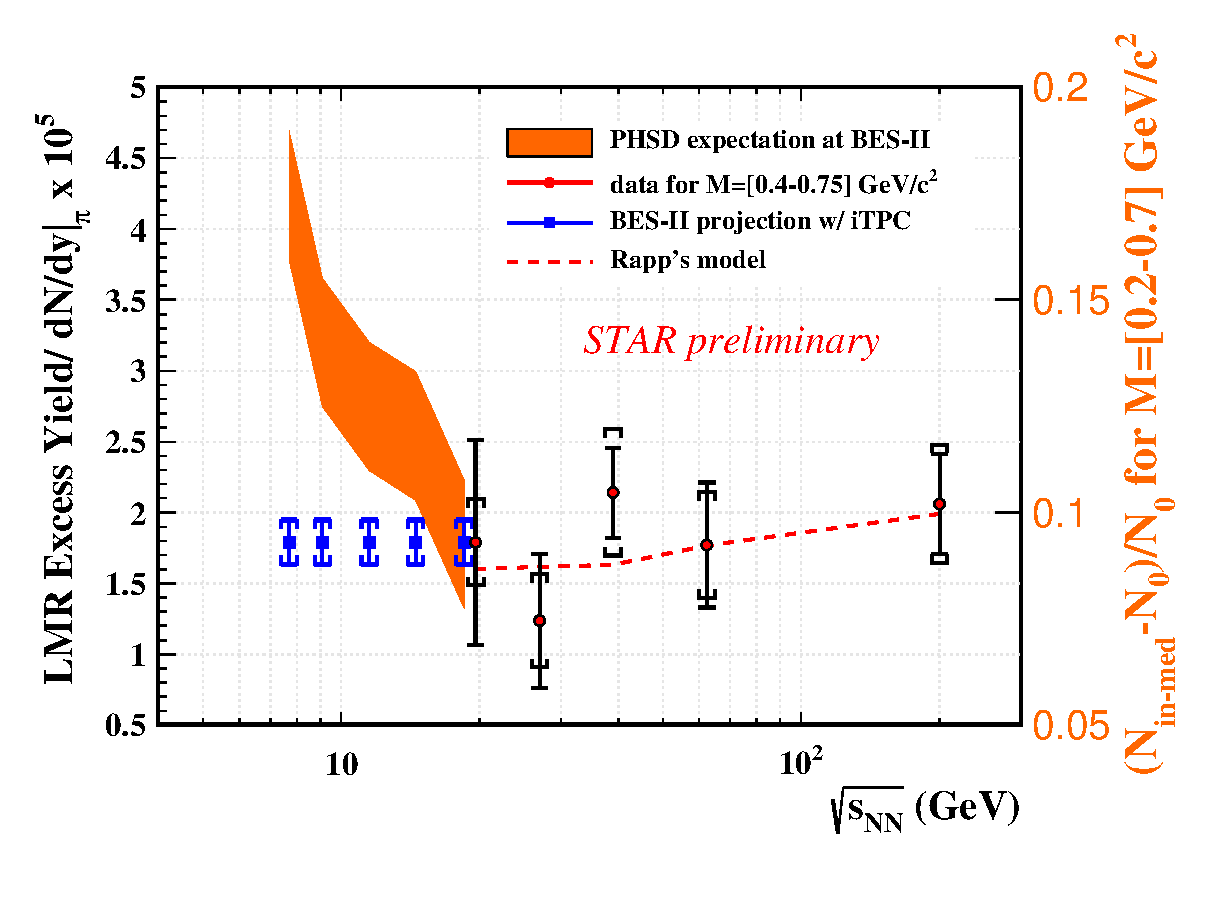
\includegraphics[width=0.5\textwidth]{outlook/iTPC_BESII_prediction.eps}
\figcaption{(Left) The dielectron excess spectrum within STAR acceptance in Au + Au minimum-bias collisions at $\sqrt{s_{NN}}$ = 19.6 GeV in the BES \uppercase\expandafter{\romannumeral1} together with the statistical and systematic uncertainty projections for BES \uppercase\expandafter{\romannumeral2} with current TPC configuration (black markers and boxes) and with iTPC upgrade (red markers and boxes). Different model calculations are also added. (Right) The $dN_{\pi}/d\eta$ normalized dielectron integrated excess yield in 0.40 $<M_{ee}<$ 0.75 GeV/$c^{2}$ for top RHIC energy and BES \uppercase\expandafter{\romannumeral1} energies, together with statistical and systematic uncertainty projections for the BES \uppercase\expandafter{\romannumeral2} energies. Model expectations from PHSD for energy below 20GeV and Rapp's model above 20 GeV are also added.}
 \label{bes2proj}
\end{figure}

\begin{figure}[htbp]
\centering
\includegraphics[width=0.46\textwidth]{outlook/proton_dndy_y.png}
\includegraphics[width=0.51\textwidth]{outlook/pion_dndy_y.png}
\figcaption{The values of $dN/dy$ for protons (circles) ~\cite{NA49proton} and pions (squares)~\cite{NA49pion} from 17.3 GeV Pb + Pb data. The closed symbols are within the coverage of the current configuration. The open symbols show the extension of coverage enabled by the iTPC and eTOF upgrades.}
 \label{forwardBaryon}
\end{figure}
